\documentclass[conference]{IEEEtran}
\usepackage{hyperref}
\IEEEoverridecommandlockouts

\usepackage{cite}
\usepackage{amsmath,amssymb,amsfonts}
\usepackage{algorithmic}
\usepackage{graphicx}
\graphicspath{ {./image/} }
\usepackage{textcomp}
\usepackage{xcolor}
\usepackage{pgfplots}
\usepackage{pgfplotstable}
\usepackage{pgf-pie}
\usepackage{subfigure}


\pgfplotsset{compat=1.18}

\def\BibTeX{{\rm B\kern-.05em{\sc i\kern-.025em b}\kern-.08em
    T\kern-.1667em\lower.7ex\hbox{E}\kern-.125emX}}
    
\begin{document}

\title{Report Title
\thanks{}
}


\author{
\IEEEauthorblockN{Nguyen Ha Khai}
\IEEEauthorblockA{Matriculation number: XXXXXXX\\
\textit{Vietnamese-German University}}
\and
\IEEEauthorblockN{Student 2}
\IEEEauthorblockA{Matriculation number: XXXXXXX\\
\textit{Vietnamese-German University}}
\and
\IEEEauthorblockN{Student 3}
\IEEEauthorblockA{Matriculation number: XXXXXXX\\
\textit{Vietnamese-German University}}
\and
\IEEEauthorblockN{\hspace{3cm}Student 4}
\IEEEauthorblockA{\hspace{3cm}Matriculation number: XXXXXXX\\
\hspace{3cm}\textit{Vietnamese-German University}}
\and
\IEEEauthorblockN{Student 5}
\IEEEauthorblockA{Matriculation number: XXXXXXX\\
\textit{Vietnamese-German University}}
}



\maketitle



\begin{abstract}
In This Part You Write The Abstract Of Your Report.
\end{abstract}

\begin{IEEEkeywords}
Note Your Keywords Here.
\end{IEEEkeywords}


\section{Introduction}
\label{sec:introduction}
In This Part You Write The Introduction Of Your Report.


\section{...}
\label{sec:second}
In This Part You Write The Second Part Of Your Report.

\subsection{Subsection 1}
\begin{itemize}
    \item bullet point 1 
    \item bullet point 2
    \item bullet point 3
\end{itemize}


\subsection{Subsection 2}
\begin{itemize}
    \item bullet point 1 
    \item bullet point 2
    \item bullet point 3
\end{itemize}

\subsection{Subsection 3}
\begin{itemize}
    \item bullet point 1 
    \item bullet point 2
    \item bullet point 3
\end{itemize}

\subsection{Subsection 4}
\subsection{Subsection 5}



\section{...}
\label{sec:Third}
In This Part You Write The Third Part Of Your Report.

\subsection{Subsection 1}
\subsection{Subsection 2}
\subsection{Subsection 3}
\subsection{Subsection 4}
\subsection{Subsection 5}











\section{Teamwork}
\label{sec:teamwork}

\begin{table}[h]
    \centering
    \caption{Task Distribution}
    \begin{tabular}{|c|p{4cm}|p{3.3cm}|}
        \hline
        \textbf{No} & \textbf{Task Description}           & \textbf{Responsible Member(s)} \\ \hline 
        1           & Task 1                         & Student 1\\ \hline
        2           & Task 2                         & Student 2\\ \hline
        3           & Task 3                         & Student 3\\ \hline
    
        
    \end{tabular}
    \label{tab:task_distribution}
\end{table}

\vspace{5em}






\begin{figure}[h]
    \centering
    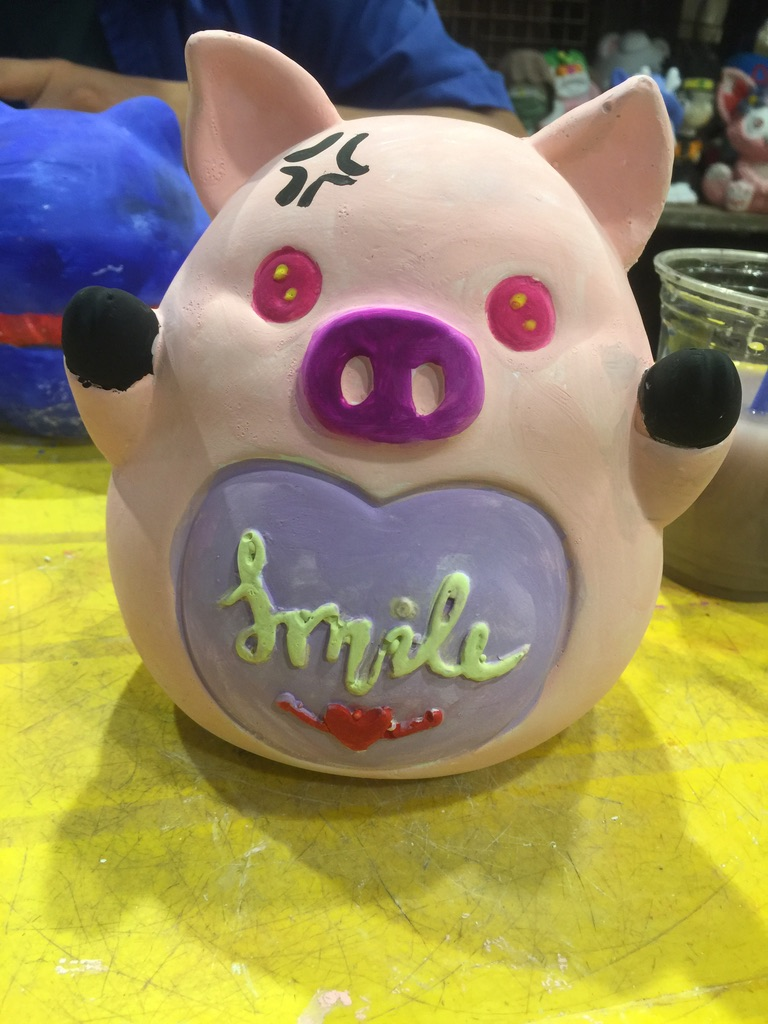
\includegraphics[width=5cm, height=4cm]{Sample.jpeg}
    \caption{Sample Image}
    \label{fig:process_flow}
\end{figure}




















\section{ Conclusions and Future Work}

In This Part You Write The Conclusion Of Your Report.



\begin{thebibliography}{00}
 
\bibitem {b1} Joshua Knowles, Weijie Zheng , “ GECCO '24 companion: proceedings of the genetic and evolutionary computation conference companion ” , Melbourne VIC Australia, pp. 1432—1459, August 2024.

\bibitem{b2} Wikipedia, ``Genetic algorithm''. Retrieved 28 January 2025, from \url{https://en.wikipedia.org/wiki/Genetic_algorithm}.

\bibitem {b3} Dinesh Bajracharya, " A review on Java hashmap and treemap ", International Journal of Engineering Applied Sciences and Technology, vol.5, pp. 134-138, May 2020.

\bibitem {b4} Lawrence Premkumar , Praveen Mohan, " Beginning JavaFX ", Apress Berkeley, CA, 26 October 2010.

\end{thebibliography}


 
 \end{document}
